% %%%%%%%%%%%%%%%%%%%%%%%%%%%%%%%%%%%%%%%%%%%%%%%%%%%%%%%%%%%%%%%%%%%%%%%%%%%%%
% %%%%%%%%%%%%%%%%%%%%%%%%%%%%%%%%%%%%%%%% Survey of the Near-Earth Environment
% %%%%%%%%%%%%%%%%%%%%%%%%%%%%%%%%%%%%%%%%%%%%%%%%%%%%%%%%%%%%%%%%%%%%%%%%%%%%%

\chapter{The Near-Earth Environment}
\label{ch_intro}

It's all about energy transfer! 

Some example citations, including a few with special characters: \cite{dai_2013}, \cite{dai_2015}, \cite{lysak_2001}. 

%There are a lot of interrelated things going on, so it's hard to describe Earth's environment one step at a time. Look at Scott's thesis -- he did this well, right? 

%Heliosphere, Magnetosphere, Ionosphere, Atmosphere?

%Current systems, convective systems, density profiles? 

%\begin{figure}
%  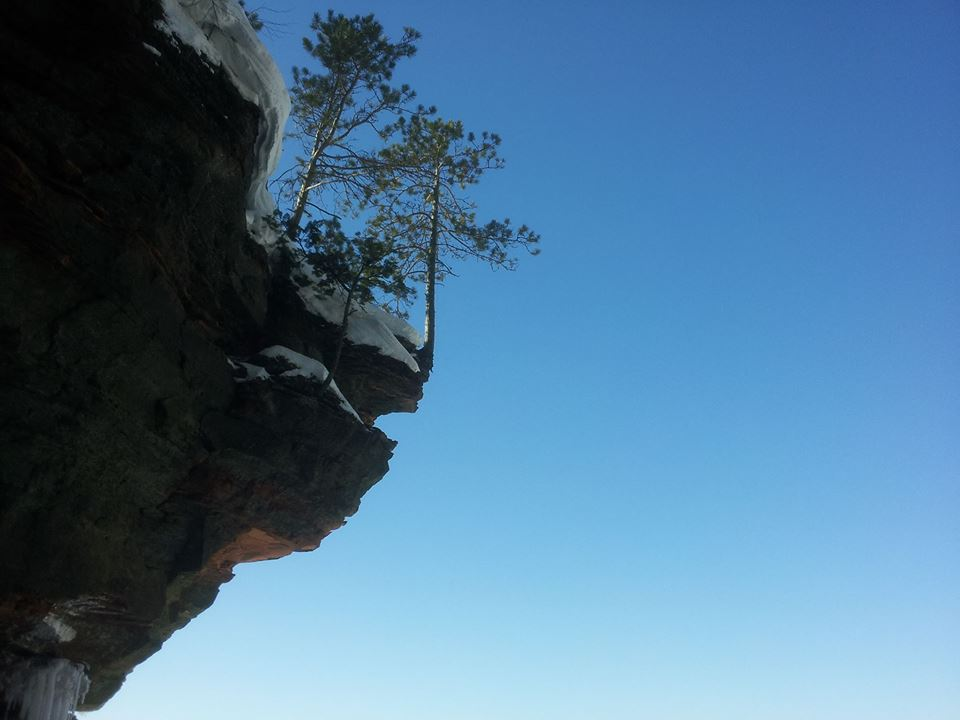
\includegraphics[width=5.75in, height=2in]{figures/image.jpg}
%  \caption{Lorem ipsum dolor sit amet, consectetur adipiscing elit, sed do eiusmod tempor incididunt ut labore et dolore magna aliqua.}
%  \label{fig_test}
%\end{figure}

Sun generates energy through nuclear reactions. 

This energy drives behavior in the near-Earth environment. 

Typical solar wind density is $\sim$ \SI{5}{/\cm\cubed}. Typical solar wind velocity at Earth is \SIrange{e2}{e3}{\km/\s}. Typical solar wind particle energy is \SIrange{1}{10}{\kilo\eV}. Density can vary by $\sim$3 orders of magnitude, and velocity by one, during times of high solar activity. CMEs can also mess with the north/south component of the interplanetary magnetic field. 

\SI{45}{\degree} angle with the Earth-Sun line, which is the \X direction. 
\footnote{We use uppercase \X, \Y, and \Z to indicate GSE coordinates: \X points from the Earth to the Sun. \Y is perpendicular to \X, and in the Sun's ecliptic plane, pointing duskwards... against Earth's orbital motion. Points north, out of the ecliptic plane. Later, we will use lowercase \x, \y, and \z to define a more-or-less analogous corodinate system with respect to Earth.}

Solar wind is what deforms Earth's magnetic field to form the magnetosphere. 

Transient solar wind phenomena, such as coronal mass ejections, are also known to be related to geomagnetic disturbances at Earth. Jesse cites here: 

R. L. McPherron. Physical processes producing magnetospheric substorms and mangetic storms. In J. A. Jacobs, editor, Geomagnetism, volume 4, chapter 7. Academic Press, 1991.

G. Rostoker. Substorms. In Handbook of the Solar-Terrestrial Environment, chapter 15. Springer-Verlag, 2007.

This might just be worth tracking down... Jesse cites several chapters: 

M. Shulz. Magnetospheres. In Handbook of the Solar-Terrestrial Environment, chapter 7. Springer-Verlag, 2007.


% papers mentioned during Yan's talk. mostly about alfven acceleration and nonlinear effects. 
% Vasyliunas 1970, 1984
% Hasegawa 1976
% Goertz 1991
% Stasiewicz et al 2000
% Haerendel 2008
% Song & Lysak 1994, 1999, 2000, 2001, 2006, 2011, 2012
% Inverted V?
% Double layers? 
% Charge holes? 



% =============================================================================
% =============================================================================
% =============================================================================
\section{The Outer Magnetosphere}

The outer magnetosphere is a region where the field lines are closed, but significantly deformed by the solar wind. 

\subsection{The Magnetopause}

\subsection{The Magnetotail}

\subsection{Cusp Regions}

% =============================================================================
% =============================================================================
% =============================================================================
\section{The Inner Magnetosphere}

In the inner magnetosphere, field lines are closed, and are approximately dipolar. 

\subsection{The Plasmasphere}

\subsection{Ring Currents}

\subsection{The Radiation Belts}

% =============================================================================
% =============================================================================
% =============================================================================
\section{Geomagnetic Disturbances}

\subsection{Storms}

\subsection{Substorms}






